Da bei vielen elektrischen und physikalischen Systemen das Rauschen zunimmt, wenn
die Frequenz $\omega$ gegen 0 strebt \cite{enet}, wird ein Lock-in-Verstärker
verwendet, um ein Signal zu verstärken. Mit dieser Technik können dann auch
Signale mit niedrigen Frequenzen detektiert werden. Um dies zu erreichen, wird die
zu messende Frequenz mit einer Referenzfrequenz $\omega_0$ moduliert. \\
\begin{figure}[h]
  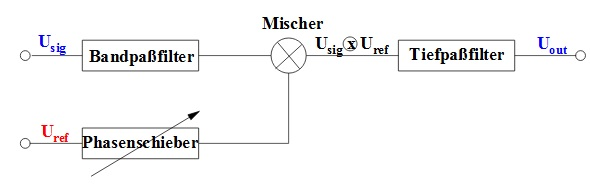
\includegraphics{Bilder/Schema.jpg}
  \caption{schematischer Aufbau}
  \label{fig:schema}
\end{figure} \\
Abbildung \ref{fig:schema} zeigt den schematischen Aufbau eines Lock-In-Verstärkers.
Das verrauschte Nutzsignal $U_{sig}$ wird zuerst durch einen Bandpass-Filter
von Rauschanteilen mit hoher beziehungsweise niedriger Frequenz befreit, bevor
es in einem Mischer mit dem Referenzsignal $U_{ref}$ mit der Frequenz $\omega_0$
multipliziert wird. Die Phasenlage $\varphi$ von $U_{ref}$ lässt sich mit dem
Phasenschieber variieren und kann so mit der Signalspannung synchronisiert werden,
sodass $\Delta\varphi =0$.
Der nachgeschaltete Tiefpass-Filter integriert das Mischsignal $(U_{sig}\times U_{ref})$
mit einer Zeitkonstanten $\tau = RC \gg 1/\omega_0$.
Rauschbeiträge, die nicht mit der Modulationsspannung synchronisiert sind, werden
hierbei herausgemittelt. Daraus ergibt sich eine zur Eingangsspannung proportionale
Ausgangsspannung $U_{out} \propto U_0 \cos(\varphi)$.

Je größer die Zeitkonstante $\tau =RC$ dabei gewählt wird, desto kleiner kann die
Bandbreite $\Delta v=1/(\pi RC)$ gewählt werden.
Der Gütefaktor, also der Energieverlust eines schwingenden Systems,
der bei Lock-In-Verstärkern erreicht wird, liegt bei Q=100000
\cite{303}.
\newpage
\begin{figure}[h]
  \centering
  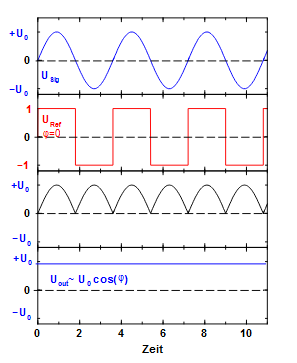
\includegraphics{Bilder/Spannung.jpg}
  \caption{Spannungsverläufe}
  \label{fig:spannung}
\end{figure}
In Abbildung \ref{fig:spannung} werden die Signalverläufe der Signalspannung
\begin{equation}
  U_{sig}=U_0\sin(\omega t)
\end{equation}
betrachtet, die durch die Rechteckspannung $U_{ref}$ moduliert wird.
Die Referenzspannung wird durch eine Fourier-Reihe mit der Form
\begin{equation}
  U_{ref}=\frac{4}{\pi}\biggl(\sin(\omega t)+\frac{1}{3}\sin(3\omega t)
  +\frac{1}{5}\sin(5\omega t)+\dots\biggr)
\end{equation}
beschrieben. Das Produkt beider Frequenzen ergibt dann:
\begin{equation}
  U_{sig}\times U_{ref} =\frac{2}{\pi}U_0\biggl(1-\frac{2}{3}\cos(\omega t)
  -\frac{2}{15}\cos(4\omega t)-\frac{2}{35}\cos(6\omega t)+\dots\biggr).
\end{equation}
Diese Formel enthält alle geraden Oberwellen der Grundfrequenz \omega.
Sind beide Frequenzen sinus-förmig, erhält man für das Produkt der beiden
die Formel:
\begin{equation}
  U_{sig}\times U_{ref}=\frac{4}{\pi}U_0 \cdot \sin^2(\omega t).
\end{equation}
Damit die Oberwellen unterdrückt werden, und eine zur Signalspannung proportionale
Gleichspannung entsteht, muss der Tiefpassfilter entsprechend eingestellt werden.
Die Gleichspannung lässt sich dann über
\begin{equation}
  U_{out}=\frac{2}{\pi}U_0
\end{equation}
beschreiben.
Sind Signal- und Referenzspannung mit $\varphi$ phasenverschoben erhält man für
die Ausgangsspannung mit
\begin{equation}
  U_{out}=\frac{2}{\pi}U_0\cos(\varphi) \label{eqn:out}
\end{equation}
wieder eine zur Signalspannung proportionale Gleichspannung. Da die Ausgangsspannung
nun von der Phasendifferenz abhängig ist, ist diese maximal bei $\varphi=0$.
